%\documentclass[11pt]{llncs} % change this around if you don't have lncs style installed
%\institute{}
\documentclass[11pt]{article}
\usepackage{enumitem}
\usepackage{listings}
\usepackage{color}
\usepackage{tabularx}

\usepackage{graphicx}
\usepackage{url}
\usepackage{sidecap}
\usepackage{epstopdf}

\def\bibfont{\scriptsize}



\usepackage{natbib}
\setlength{\bibsep}{0.0pt}

\lstset{basicstyle=\scriptsize\sffamily}
%\lstset{language=Assembler}[avr8avra] % not standard
\lstdefinestyle{customasm}{
  morekeywords={adc,adiw,asr,brts,brcs,brhs,brne,cbr,clh,clr,clt,cp,cpi,dec,eor,ldi,lpm,lsl,nop,mov,or,rcall,ret,seh,set,subi,swap,rjmp},
  morecomment=[l][\color{blue}]{;}
}
\lstset{style=customasm}

\begin{document}
\title{Speed and size-optimized implementations of the PRESENT cipher for tiny AVR devices}
%\title{\textbf{PRESENT Cipher for tinyAVR Architectures}}

\author{}
\date{}
\maketitle

\begin{abstract}
\textbf{This paper presents high-speed and low-size assembly implementations of the 80-bit version of the PRESENT cipher for the AVRtiny family of microcontrollers. We report new speed and size records for our implementation, with the speed-optimized version achieving a full encryption in 8721 clock cycles and the size-optimized version compressing the cipher down to 280 bytes; the previous state of the art for AVRtiny achieved 10723 clock cycles for encryption with a size of 936 bytes. Along with the two implementation extrema (speed \& size optimized versions), we offer insight into techniques and representations that show the speed/area tradeoffs and provide intermediate solutions for various configurations.\\Keywords: PRESENT, AVR, tinyAVR, software implementation.}
\end{abstract}
\section{Introduction}
Modern society is constantly witnessing an extensive and large scale deployment of tiny computing devices. Information processing and wireless communication are being thoroughly integrated into everyday objects and activities, developing a large distributed mobile infrastructure and ushering in the era of ubiquitous computing. RFID tags attached to products, cardiac pacemakers, fire-detecting sensor nodes and the like need to operate \emph{securely} under particularly \emph{restricted conditions}, namely low battery life, small processing power and bandwidth-demanding ad-hoc network protocols. To achieve sustainable security in this new landscape, researchers have developed new cryptographic primitives and techniques, namely lightweight cryptographic ciphers such as PRESENT~\cite{bogdanov2007present}, Klein~\cite{gong2012klein}, LED~\cite{guo2011led} and others.

The majority of these ciphers was designed with hardware performance in mind, leaving most software implementations relatively inefficient. For instance, the AVR-Crypto-Lib~\cite{avr_crypto_lib} often resorts to C language implementations, resulting in 100k clock cycles for a single encryption with PRESENT.
AVR microcontrollers are often encountered regarding the Internet of Things and ubiquitous computing, and moreover serve as a good model of a limited instruction set architecture, thus they are an interesting platform on which to enable and optimize lightweight ciphers.
The University of Leuven has initiated a project to draft efficient assembly implementations of various lightweight ciphers on resource-constrained AVR devices to make fair comparisons about their relative efficiency. The contribution by Eisenbarth~\cite{eisenbarth2012compact} achieves an encryption in roughly 11.000 clock cycles.

\textbf{Our contribution.} This paper describes a speed-optimized and a size-optimized implementation of the PRESENT cipher on the ATtiny45, with the aid of algorithmic improvements and efficient programming techniques. Our speed-optimized version improves the state of the art~\cite{eisenbarth2012compact} by 18\%, while the size-optimized version is 70\% smaller than the smallest known implementation~\cite{eisenbarth2012compact}.\\
Algorithmic improvement:
\begin{itemize}[nolistsep]
  \item A merged SP layer, \emph{i.e.} combining the substitution and permutation layer of the cipher in order to construct lookup tables that remove the time-consuming permutations~\cite{gong_code}. This improvement constitutes the core of the achieved speed improvement.
\end{itemize}
Programming improvements:
\begin{itemize}[nolistsep]
  \item Squared S-Box representations, \emph{i.e.} S-Boxes which are custom-made for fast access in the AVR 8-bit architecture, also used by Eisenbarth~\cite{eisenbarth2012compact}.
  \item Compact S-Box representations, \emph{i.e.} minimal footprint S-Boxes that reduce the implementation size.
  \item Minimal key register rotations, allowing the key update procedure to complete in fewer instructions.
  \item Memory access optimizations, grouping memory transactions to improve speed.
  \item Algorithm serialization, by keeping part of the state in SRAM while we operate on fewer registers.
  \item Indirect register access to let loops drive repeated operations on CPU registers.
  \item Use of the stack to store intermediate values to avoid more dedicated registers.
  \item Code restructuring and efficient procedure callings.
\end{itemize}
We note that some of the improvements are interoperable and can be combined to provide the ``golden ratio" between speed and size, depending on the external requirements.\\
\textbf{Paper organization.} The organization of the paper follows. Section 2 provides an introduction to the AVR architecture, including the capabilities and limitations of AVRtiny microcontrollers. Section 3 focuses on high-speed implementation of the PRESENT cipher, regarding efficient S-Box representations and lookup tables. Section 4 describes various techniques that produce a very compact version of the cipher. Section 5 provides the final benchmarking results and conclusions.

\section{Background}
\subsection{PRESENT cipher}
 PRESENT~\cite{bogdanov2007present} is an ultra-lightweight, 64-bit symmetric block cipher, using 80-bit or 128-bit keys.
It is based on a substitution/permutation network and it is named as a reference to Serpent~\cite{anderson1998serpent} due to its similar constructs.
As of 2012, PRESENT (among other ciphers) was adopted by ISO as a standard for a lightweight block cipher (ISO/IEC 29192-2:2012~\cite{present_iso}). The full algorithm has so far been resistant to attempts at cryptanalysis, although the most successful attack has shown that up to 15 of its 31 rounds can be broken with $2^{35.6}$ plaintext-ciphertext pairs in $2^{20}$ operations~\cite{abed2012biclique,collard2009statistical,nakahara2009linear}.

PRESENT uses exclusive-or as its round key operation, a 4-bit substitution layer, a 4-bit period bit position permutation network in 31 rounds and a final round key operation.
Key scheduling is a combination of bit rotation, S-Box application and exclusive-or with the round counter.
%We chose PRESENT as a cipher to work on within a project to write and optimize AVR crypto code %because we deemed it extremely well-suited for a simple microcontroller, and felt it was within our %grasp to implement and optimize correctly within the allotted time.
Constructs found in PRESENT are also encountered in SPONGENT~\cite{bogdanov2011spongent}, in hash function constructs based on block ciphers proposed by Hirose \cite{bogdanov2008hash,hirose2005provably,hirose2006some} (H-PRESENT) and in the derivative SMALLPRESENT \cite{leander2010small}, so the optimizations presented here can also be of interest with respect to the implementations of these ciphers. In our approach, we have implemented PRESENT for the recommended 80-bit key size in AVR assembly in two versions, optimized for maximal speed and minimal size.
(Support for 128-bit keys was also added to the size-optimized implementation as the required extra registers became available through optimizations, but we will focus on the implementation of the variant with 80-bit keys.)

\subsection{PRESENT algorithm.}
The cipher's key register is supplied with the 80-bit cipher key and in every encryption round the first 64 bits of the 80-bit key register form the round key.
To encrypt a single 64-bit block, during each encryption round, PRESENT applies a XOR with the current round key followed by a substitution and a permutation layer.
The substitution layer applies nibble-wise (4-bit) S-Boxes to the state, while the permutation layer re-arranges the bits in the state following a 4-bit period.
Key scheduling is done by rotating the key register 61 bit positions to the left, applying the S-Box to the top nibble of the key register and XORing bits 15 through 19 with the round counter.
There is a total of 31 such rounds and finally the round key is applied one last time 
(Figure~\ref{present_schematic}.).


\begin{figure}[h]
	\label{present_schematic}
	\centering
	 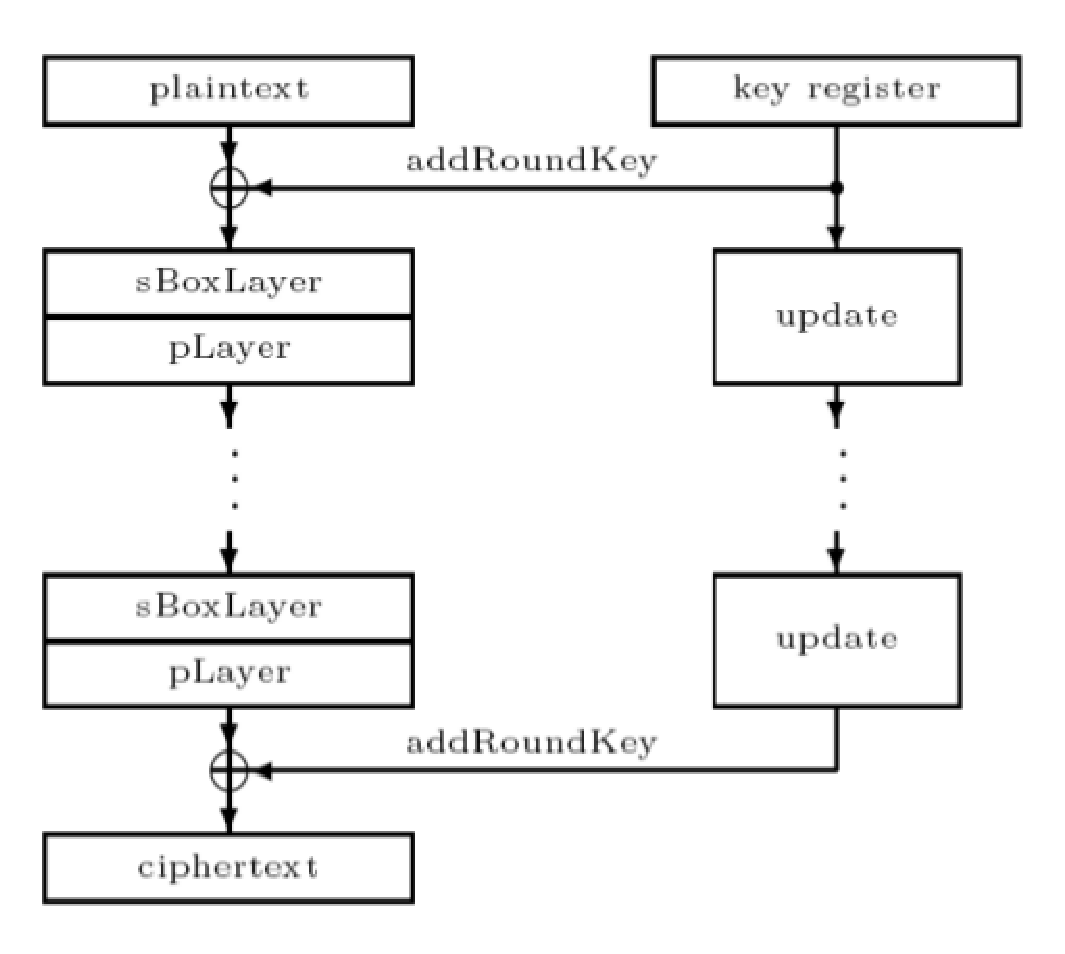
\includegraphics [width=0.6\textwidth]{present.eps}
\caption{\footnotesize Schematic of the PRESENT cipher. It consists of 31 rounds, including substitution, permutation and key update.}
\end{figure}
\subsection{The 8-bit family of tinyAVR Microcontrollers}
Atmel offers a wide range of 8-bit microcontrollers, including high performance devices (ATxmega), mid-range devices (ATmega) and low-end devices with limited memory, storage and processing power (ATtiny). Common applications of AVR microcontrollers include smart cards, motor control systems, medical applications et cetera. 

Our focus is on the resource-constrained ATtiny architecture, which typically features less than 1 kilobyte of static RAM (SRAM) and flash storage ranging from 1 to 8 kilobytes. The architecture uses 32 general-purpose registers, \textit{R0}-\textit{R31}.

Several registers have special characteristics, namely registers \textit{R0} through \textit{R15} can only be accessed by instructions that provide an immediate value as an operand, \emph{e.g.} you cannot perform memory access from these registers.
In addition, registers \textit{R27:R26} (denoted as \emph{X}), registers \textit{R29:R28} (denoted as\emph{Y}) , and registers \textit{R31:R30} (denoted as \emph{Z}) can access the SRAM.
The \emph{Y} register can be used for indirect register addressing, and the \emph{Z} register can access the flash storage as well as be used for indirect jumps and calls.
Instructions using these 3 pointer registers also allow post-increment and pre-decrement of the pointer.
At all times, the 6 special registers can be utilized as general-purpose registers.

The ATtiny instruction set consists of the basic 90 instructions, found in all AVR architectures. However, due to the limited size of its core, it does not support the extended instruction set which includes multiplication, in contrast with the ATmega architecture.\\
\textbf{ATtiny configuration.} We perform all simulations on ATtiny45, which has a maximum clock frequency of 20 MHz, 256 bytes of SRAM and 4 KB of flash storage.\\
\textbf{Radix-$2^8$ representation.} The PRESENT cipher requires representing integers of size 64 and 80 bits. Thus, we split the number into 8-bit components, using radix-$2^8$ and an $m$-bit integer is represented as $n=\lceil{m/8}\rceil$ bytes $(x_0,x_1,\dots,x_{n-1})$ such that $x=\sum_{i=0}^n{x_i 2^{8*i}}$.

\section{High-speed implementation}

\subsection{PRESENT S-Box \& Player implementation}\label{sbox}
In this section we examine the S-Box of the PRESENT cipher from the speed perspective, using lookup tables, and we offer several variations, utilizing the time-space tradeoff. We analyze the \emph{original S-Box}, identify its performance issues (section \ref{osbox}) and suggest two possible lookup table representations (with 8 and 16 bytes respectively). Subsequently, we expand it to the faster, yet space-demanding (256 bytes) \emph{Squared S-Box} (section \ref{ssbox}). In the last section, we examine the \emph{combination of the S-Box and the permutation layer}, resulting in a very large lookup table (1024 bytes) that substantially boosts performance (section \ref{msbox}).

\subsubsection{Original S-Box}\label{osbox}
The original S-Box, presented by Bogdanov et al.~\cite{bogdanov2007present} consists of 16 different substitutions, each with a 4-bit input and a 4-bit output, as shown in Table~\ref{original_sbox}.
\begin{table}[h]
\footnotesize
\centering
\begin{tabular}{| c | c  | c | c | c  | c | c | c  | c | c | c  | c | c | c  | c | c | c |}
\hline
  x & 0 & 1 & 2 & 3 & 4 & 5 & 6 & 7 & 8 & 9 & A & B & C & D & E & F   \\
\hline
  S[x] & C & 5 & 6 & B & 9 & 0 & A & D & 3 & E & F & 8 & 4 & 7 & 1 & 2   \\
\hline
\end{tabular}
 \caption{\footnotesize The original S-Box of the PRESENT cipher.}
 \label{original_sbox}
\end{table}\\
\textbf{Representation.} If we aim for a particularly small size footprint, it is possible to use either a \emph{packed} or an \emph{unpacked} representation of the original S-Box. The \emph{unpacked} version stores the lookup table in 16 bytes, where every 4-bit input to 4-bit output substitution is stored using 8 bits of space (\emph{i.e.} there exists redundancy in the representation) and is the same with the original S-Box. The \emph{packed} version, stores \emph{two} 4-bit input to 4-bit output substitutions using 8 bits, \emph{i.e.} without any redundancy, resulting in an 8 byte lookup table. \\
%\begin{table}[h]
%\centering
%\scriptsize
%\begin{tabular}{| c | c  | c | c | c  | c | c | c  | c | c | c  | c | c | c  | c | c | c |}
%\hline
%  x & 00 & 01 & 02 & 03 & 04 & 05 & 06 & 07 & 08 & 09 & 0A & 0B & 0C & 0D & 0E & 0F   \\
%\hline
%  S[x] & 0C & 05 & 06 & 0B & 09 & 00 & 0A & 0D & 03 & 0E & 0F & 08 & 04 & 07 & 01 & 02   \\
%\hline
%\end{tabular}
% \caption{\footnotesize The unpacked representation of the original S-Box, using 16 bytes. Each table column represents a single substitution.}
% \label{unpacked_sbox}
%\end{table}\\
\begin{table}[h]
\centering
\footnotesize
\begin{tabular}{| c | c  | c | c | c  | c | c | c  | c | c | c  | c | c | c  | c | c | c |}
\hline
  x & 01 & 23 & 45 & 67 & 89 & AB & CD & EF   \\
\hline
  S[x] & C5 & 6B & 90 & AD & 3E & F8 & 47 & 12   \\
\hline
\end{tabular}
 \caption{\footnotesize The packed representation of the original S-Box, using 8 bytes. Each table column represents two substitutions. This would give a size optimization of 8 bytes to begin with, but considerations for unpacking code apply. (See Section~\ref{sbox_packing}.)}
 \label{packed_sbox}
\end{table}\\
\textbf{Performance.} The core performance issue regarding the 4-bit S-Box is the penalty in accessing it, if stored in a lookup table. The AVR architecture is designed to enable fast access for 8-bits at a time. Thus, a lookup table with of the original S-Box is rather small (16 bytes for an unpacked version, 8 bytes for a packed one), but it is also rather inefficient (speed-wise) due to the overhead operations that need to take place before and after each table lookup. The packed S-Box (Table~\ref{packed_sbox}) is the least speed-efficient variant, since after the lookup we always have to extract the upper or lower half. This issue is not encountered in the unpacked version, which makes better use of the AVR 8-bit architecture. However, performance is not optimal  due to the fact that we only substitute 4 bits at a time, while we use 8-bit operations, \emph{i.e.} the redundant representation results in more memory accesses than needed. 

\subsubsection{Squared S-Box}\label{ssbox}
A solution to the aforementioned performance problem is to construct a new lookup table that:\emph{(a)} is custom made for the 8-bit AVR architecture, like the unpacked S-Box and \emph{(b)} uses a non-redundant representation similar to the packed S-Box.\\
\textbf{Representation.} In Table~\ref{squared_sbox}, we demonstrate a \emph{Squared S-Box}, which uses an 8-bit input and produces an 8-bit output. Within an 8-bit space, we can contain two 4-bit substitution values and the number of possible substitution values is 16, thus the total size of the lookup table is $16*16=256$ bytes. As a result, there is no need for overhead computation and the substitution consists of a single lookup. This approach has also been followed before by Eisenbarth~\cite{eisenbarth2012compact}\\
\begin{table}[h]
\footnotesize
\centering
\begin{tabular}{| c | c  | c | c | c  | c  | c | c | c  | c | c | c |}
\hline
  x & 00 & 01 & 02 & 03  &  $\dots$  & 0C & 0D & 0E & 0F   \\
\hline
 S[x] & CC & C5 & C6 & CB & \dots & C4 & C7 & C1 & C2   \\
\hline
  x & 10 & 11 & 12 & 13  &  $\dots$  & 1C & 1D & 1E & 1F   \\
\hline
 S[x] & 5C & 55 & 56 & 5B & \dots & 54 & 57 & 51 & 52   \\
\hline
  \vdots & \vdots & \vdots & \vdots & \vdots  &  $\dots$  & \vdots &\vdots & \vdots & \vdots   \\
\hline
  x & F0 & F1 & F2 & F3  &  $\dots$  & FC & FD & FE & FF   \\
\hline
 S[x] & 2C & 25 & 26 & 2B & \dots & 24 & 27 & 21 & 22   \\


\hline
\end{tabular}
 \caption{\footnotesize The 256-byte Squared S-Box. It substitutes one byte at a time, without any overhead or redundancy.}
 \label{squared_sbox}
\end{table}
\textbf{Performance.} The Squared S-Box described, is an efficient and viable solution with respect to the cipher's substitution layer. It is custom made for the 8-bit AVR architecture and allows us to perform byte substitutions with a single flash memory lookup. Furthermore, it is relatively size-efficient, consisting of 256 bytes, thus, it can be transfered to ATtiny45 SRAM from flash memory during the initialization process of the algorithm. The memory transfer is viable, since ATtiny45 possesses only 256 bytes of SRAM and it will reduce the lookup cost by 33\%, \emph{i.e.} to perform a lookup, the software will use the \texttt{ld} instruction (load from SRAM - 2 clock cycles), instead of  the \texttt{lpm} instruction (load from flash memory - 3 clock cycles) and thus, each lookup will cost 1 cycle less. Given the fact that the block size of the PRESENT cipher is 64 bits, it requires $64/8=8$ lookups per round. The cipher consists of 31 rounds and an implementation using SRAM will result in $8*31=248$ clock cycles reduction for a full encryption. The only processing penalty consists of a 256 byte transfer from flash storage to SRAM which occurs only once, preferably in the beginning or setup phase.

\subsubsection{Merged SP lookup table}\label{msbox}
Although the Squared S-Box lookup table solution is viable for the PRESENT cipher, we need to stress the fact that the PRESENT cipher possesses a complex permutation layer, requiring a large number of shift and rotate operations. The AVR architecture is not capable of performing fast shifts and rotations (compared for instance with the ARM11 processors which can do shifts and rotations for free),  \emph{i.e.} an $n$-bit shift requires $n$ clock cycles, and thusly we have to look for alternatives.
In this direction, work by Hutter \& Schwabe~\cite{hutternacl} on ATmega\footnote{Benchmarking was performed on ATmega2560.} suggested the usage of multiplications instead of rotations/shifts, however this is not viable on ATtiny due to the fact that they do not possess native multiplication instructions.\\
\textbf{Representation.} The fastest approach that we identified for the permutation layer is the idea developed by Zheng Gong and Bo Zhu~\cite{gong_code,gong2009towards}. Due to the adaptation of this novel approach in the AVR architecture, we are able to improve performance over the state of the art~\cite{eisenbarth2012compact}. Specifically, Gong \& Zhu exploited the internal structure of the permutation layer, \emph{i.e.} the fact that every output of a 4-bit S-Box will contribute one bit to the cipher (the underlying pattern for the permutation is the following: $for$ $k:old$ $position,$ $l:new$ $position,$ $l=f(k)=16(k mod 4)+(k div 4)$ ). Thus, the first 2 bits of the output are derived from the first two 4-bit S-Boxes, i.e. from the first byte of the previous state. \\
Using these observations, they crafted four 256-byte lookup tables (1024 bytes in total) that \emph{merge} the S-Box and the permutation layer and as a result, the whole SP network is performed via table lookups.\\
\textbf{Performance.} The 1024 byte lookup tables eliminate the need for an independent permutation layer, providing us with the fastest available solution. On the downside, we have to perform one lookup for every two bits, resulting in 32 lookups for a 64-bit state (compared to the Squared S-Box that required only 8 lookups for a 64-bit state). Moreover, we need 1024 bytes to store the tables, thus it is not possible to transfer them to the SRAM. The 33\% speedup obtained in section \ref{ssbox} is only possible in an AVR microcontroller with at least 1024 bytes of internal\footnote{Additional external SRAM is not an option, since it is at least as slow as flash memory.} SRAM, for instance ATtiny1634.\\
\textbf{Time-memory tradeoff.} We conclude the discussion on the substitution/permutation techniques by presenting all the proposed solutions (original, squared or merged S-Box) in the form of a spectrum diagram. Depending on the requirements, resources or limitations induced, one may choose the most suitable representation, with the aid of the following spectrum diagram.
% TODO reviewer suggested we replace this with a table
\begin{figure}[h]
\centering
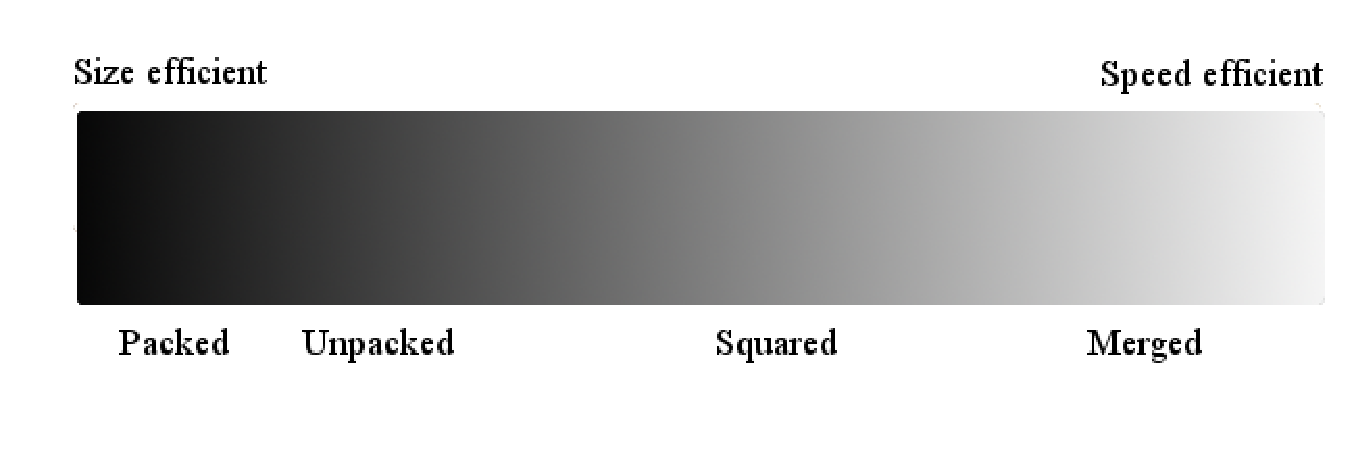
\includegraphics[scale=0.3]{spectrum}
\caption{\footnotesize The available S-Box representations, shown on the size-speed spectrum.}
\end{figure}
%\begin{table}[h]
%\footnotesize
%\centering
%\begin{tabular}{| c | c  | c | c | }
%\hline
%  Representation & Flash (bytes) & SRAM (bytes) & Comments  \\
%\hline
%  Packed S-Box & 8  & 0-8 & Compact, slow   \\
% \hline
%  Unpacked S-Box & 16  & 0-16 & Compact, slow   \\
%\hline
%  Squared S-Box & 256  & 0-256 & Medium speed and size   \\
% \hline
 % Merged SP & 1024  & 0-1024 & High speed and size  \\
 

%\hline
%\end{tabular}
%\caption{\footnotesize Comparison of S-Box representations. Note that all representations are viable on ATtiny45 when implemented with flash storage. In the case that the tables are transfered to SRAM for faster %lookups, only packed, unpacked and squared are viable on ATtiny45 due its SRAM size (256 bytes). Merged SP on SRAM is viable on ATtiny1634 (featuring 1KB of SRAM). }
%\end{table}
\subsubsection{Memory optimizations for lookup tables}
All the aforementioned solutions with respect to substitution and/or permutation rely heavily on lookup tables. In order to decrease the computational penalty of the table lookups, we performed several code-level optimizations. Below, we demonstrate the code required to perform a single table lookup from flash memory.
\begin{verbatim}
mov ZH , high_part_of_address; 
mov ZL , low_part_of_address; 
lpm register , Z ;
\end{verbatim}
The lookup operations consists of two \texttt{mov} and one \texttt{lpm} instruction. Memory is addressed using 16 bits pointers, so the first \texttt{mov} loads the high part, while the second \texttt{mov} loads the table index that will be accessed.\\
\textbf{Table alignment.} We aim to keep the changes required in the high part (\texttt{ZH}) to a minimum. Thus, we align the four 256-byte tables required for the merged SP approach in section \ref{msbox} such that they can be accessed by using only the  low part (\texttt{ZL}) register as an index and keeping \texttt{ZH} unchanged. Elaborating, the four lookup tables start from \texttt{0x0600, 0x0700, 0x0800, 0x0900} respectively and thus, the 8 high bits of the address part (\texttt{0x06, 0x07, 0x08, 0x09}) remain the same while the 8 low bits are sufficient to act as the table index, ranging from 0 to 255 (\texttt{0x00} to \texttt{0xFF}). \\
\textbf{Memory access grouping.} Performing two lookup operations in two different tables requires a total of 10 clock cycles (2 \texttt{mov} to change the high part of the operation, 2 \texttt{mov} to change the index and 2 \texttt{lpm} to perform the actual lookup). However, performing two lookup operations on the \emph{same table} requires a total of 8 clock cycles (2 \texttt{mov} for the index, 2 \texttt{lpm} for the lookup), since the high part of the memory address remains the same. Thus, we 
we try to perform the maximum amount of grouped table lookups, given the limited number of registers, since within each group, \texttt{ZH} remains the same. For instance the following sequence of operations, \emph{ lookupTable1(i), lookupTable2(k), lookupTable1(j), lookupTable2(m)} will transform to \emph{ lookupTable1(i), lookupTable1(j), lookupTable2(k), lookupTable2(m)} in order to group memory access.
\subsection{Key update implementation}
This section focuses on implementing the key scheduling/update process of the PRESENT cipher efficiently. The key update function of the PRESENT cipher consists of three operations, namely, key rotation, key substitution and key XOR the round counter. We present the optimizations performed in the following subsections.
\subsubsection{Key rotation}
The algorithm specifies that the key must be rotated by 61 bits to the left. Given the fact that rotations/shifts are computationally expensive in the AVR architecture, we transform 61 left rotations to 19 right rotations, which can be further reduced to 16 right rotations and 3 right rotations. The 16 right rotations can be easily performed by using the \texttt{mov} instructions on register level, i.e. rotate all the bits inside a register by moving the contents to the previous register used in our representation, an approach which is preferable to single rotations via the bit-level instructions. Only the 3 remaining rotations are carried out with the logical instructions for right rotation and shifting (\texttt{ror} and \texttt{shr}).

\subsubsection{Key substitution}
The highest 4 bits of the 80-bit key used by the PRESENT cipher, must be substituted via the S-Box. To avoid 4-bit memory access or redundancy (section \ref{osbox}), we construct a special-purpose Squared S-Box that substitutes the 4 high bits of the 8-bit input, while the low 4 bits remain unchanged. The resulting table applies a substitution operation on the upper nibble which takes only a single lookup operation. Should we encounter space constraints, it is possible to replace the Squared S-Box with the original, unpacked one; the key substitution occurs only once per round, so the performance loss incurred by the unpacked S-Box is relatively small. 

%\begin{table}[h]
%\footnotesize
%\centering
%\begin{tabular}{| c | c  | c | c | c  | c  | c | c | c  | c | c | c |}
%\hline
%  x & 00 & 01 & 02 & 03  &  $\dots$  & 0C & 0D & 0E & 0F   \\
%\hline
% S-Box[x] & C0 & C1 & C2 & C3 & \dots & CC & CD & CE & CF   \\
%\hline
%  x & 10 & 11 & 12 & 13  &  $\dots$  & 1C & 1D & 1E & 1F   \\
%\hline
% S-Box[x] & 50 & 51 & 56 & 5B & \dots & 5C & 5D & 5E & 5F   \\
%\hline
%  \vdots & \vdots & \vdots & \vdots & \vdots  &  $\dots$  & \vdots &\vdots & \vdots & \vdots   \\

%\hline
%  x & F0 & F1 & F2 & F3  &  $\dots$  & FC & FD & FE & FF   \\
%\hline
 %S-Box[x] & 20 & 21 & 22 & 23 & \dots & 2C & 2D & 2E & 2F   \\
%\hline


%\end{tabular}
% \caption{\footnotesize Special-purpose Squared S-Box for key substitution, operating only on the high 4 bits of the input.}
% \label{key_sbox}
%\end{table}

\subsubsection{Key exclusive OR operation} \label{key_xor}
The algorithm specifies that the key bits 15, 16, 17, 18, 19 must be XORed with the round counter. The issue is that -under the current representation- bits 0$\dots$7 will be stored in register0, bits 8$\dots$15 will be stored in register1 and bits 16$\dots$23 will be stored in register2. As a result parts of the round counter need to be XORed with different parts of two separate registers, namely the counter needs to be XORed with both register1 and register2. Similarly to \cite{eisenbarth2012compact}, we perform the XOR operation before the key rotation, thus the bits that are operated on are bits 34,35,36,37,38 which span a single register (using the previous representation, they are located in register4 ). This restructuring, \emph{i.e.} performing the XOR operation before the key rotation does not affect the outcome or security of the algorithm. 


% NOTE: This is not a valid/verified section yet - we only present thoughts on the possibility of bitslicing. %To be reconsidered.\\
%Bitslicing has been performed before for PRESENT ~\cite{bitslice}.In order to perform bitslicing in %AVR, there is need for a large amount of SRAM, e.g. for a fully-blown bitslicing, we need 8*64=512 %bytes of SRAM. With this approach we perform 64 encryptions in bitsliced form and we no longer %need the permutation layer. On the downside, there will traffic between registers and SRAM and also, %we cannot use lookup tables for the substitution layer and thus, we have to implement the S-Box with %boolean functions that operate on each state bit.

\section{Size-optimized implementation}

Here we will list some of the size improvements we were able to apply to the PRESENT algorithm.
While these modifications make the algorithm operate more slowly, the reduction in size would allow the cipher to be included in microcontrollers with smaller available code area.
Our version requires 132 AVR instructions (264 bytes of code) for both the encryption and decryption routines, plus two times 8 bytes for packed tables of S-Box values at memory addresses \texttt{0x100} and \texttt{0x200}.
We believe this should be sufficiently small for the code to be included in an AVR machine with 1K of available Flash storage, while still allowing over half of the available area to be devoted to application-specific code.

Unfortunately, every opcode in the AVR instruction set is 16-bits wide, so there is nothing to be gained from exchanging any instructions for equivalent smaller ones (such as for example \textit{add Rd, 1} being more concisely expressed as \textit{inc Rd} on x86 machines).
Furthermore the AVR employs a Harvard architecture, where there is a strict separation between data and code memory; this prevents us from dynamically computing new opcodes in memory to be executed later.
Finally we note there are no `bulk' instructions which operate on several registers at once.

However, we do have access to some instructions that are specific to the AVR architecture and are uniquely suited to making parts of the code more condensed by virtue of their expressiveness, such as the \textit{swap} and \textit{cbr} instructions.
We also have all kinds of branching instructions at our disposal.
These instructions branch based on values in the state register (SREG), which we can explicitly or implicity modify.
We can use the stack to make procedure calls or as temporary storage, and finally have the powerful option of adressing the CPU registers indirectly through the Y register.

\subsection{Serialization and SRAM use}
The greatest size optimization we have implemented is serialization of the algorithm, keeping most of the state in SRAM while we operate on fewer dedicated registers.
This reduces the instruction count on all parts of the round update procedure except for key scheduling.

We have chosen to keep 4 bytes of state in registers at a time, as we believe it allows us to apply the permutation layer of the algorithm in software with the most size-efficiency.
Using even fewer state bytes in registers might allow for greater size reductions in other areas of the code, but applying the permutation layer may turn out to be more troublesome in that case.

By requiring only 4 dedicated registers to keep a partial block state, and 6 to keep the rest of the algorithms state, we were left with exactly 16 of the 32 general purpose registers available to keep the key register (as we rely on the 6 registers for X,Y,Z to navigate the SRAM, indirectly addressed registers and flash storage respectively.)
This means support for 128-bit keys was able to be added to the implementation at no extra cost.
%We would of course welcome efforts from the community to disprove this assumption.

\subsection{S-Box packing}\label{sbox_packing}
The PRESENT S-Boxes work on 4-bit nibbles, but defining a table of nibbles in the code at first seemed less size-efficient than packing the nibbles into bytes to be unpacked.
This would save 8 bytes per S-Box table to start with, but we need 5 to 8 instructions in stead of a \textbf{ld} (load) depending on whether or not we care about timing attacks to unpack the nibbles which diminishes the size benefit to 2 bytes of code. See Figure~\ref{unpacking_code} and Table~\ref{packed_sbox}.

The S-box construct replaces a single low nibble in the output.
The simplest and most size-efficient way to apply it to a byte in code consists of 1) calling it, 2) swapping the resulting nibbles, 3) calling it again for the other nibble and then 4) swapping the nibbles back.
We can call this code starting from step 2 to apply the S-box to only the high nibble of a byte, as is required when scheduling new round keys.
%We consider this a fair loss for our optimization strategy, and also see an upside: having the S-Boxes unpacked as data improves throughput and makes the encryption and decryption code smaller to distribute separately.
%We decided 2 bytes of area reduction just wasn't worth the other losses.
%The packed table approach is therefore only beneficial when we require encryption and decryption routines in the target application, in which case it would save the remaining 6 bytes.

\begin{figure}
\begin{lstlisting}
	unpack_sBox:
		asr ZL                ; halve input, take carry
		lpm SBOX_OUTPUT, Z    ; get S-Box output
		brcs odd_unpack       ; branch depending on carry
	even_unpack:
		swap SBOX_OUTPUT      ; swap nibbles in S-Box output
		rjmp unpack
        odd_unpack:
                nop                   ; guard against timing attacks
                nop
        unpack:
                cbr SBOX_OUTPUT, 0xf0 ; clear high nibble in S-Box output
	\end{lstlisting}
	\caption{\footnotesize Unpacking bytes into nibbles in a constant cycle count takes us 8 instructions whereas unpacking unpacked nibbles takes us only 1. The net gain is only 2 bytes of code.}
\label{unpacking_code}
\end{figure}


\subsection{Permutation layer}
The code to apply the bit position permutation to the state in software borrows heavily from the AVR implementation of PRESENT drafted in Leuven by Eisenbarth et al.~\cite{eisenbarth2012compact}.
Since the permutation follows a 4-bit period in the input, their choice to use 4 bytes of I/O when rotating bits off of registers into corresponding new positions seems quite efficient.
In the Leuven implementation one bit is rolled off from 4 state registers into one output register and this block is done twice, completing one output byte.
%It has made ingenious use of the side-effect that both the input and the output are being rotated, allowing the operation to be reversed depending on the offset at which the procedure is called.

This implementation of the permutation layer requires availability of 4 bytes of temporary storage for half of the permuted state, which we save to the stack before applying the permutation to the other 4 bytes of the state.
The construct in Figure~\ref{sreg_redo} allows the implementer to let a block of code be executed twice, while allowing them to take control of the machine before, after and in between these code blocks.
As you can see this takes 4 instructions, whereas a \textit{rcall}, \textit{ret} construction would take us only 3, but this construct doesn't use the stack which means we can keep our intermediate values there rather than requiring 4 more dedicated registers or make more complicated use of the SRAM.

%In our implementation this construct has been applied to the permutation layer procedure (which requires intermediate storage) to save a few instructions while arranging its temporary state into its final state, and make use of fewer dedicated registers.

%Using fewer dedicated registers also requires fewer dedicated instructions to directly interact with them, which means reduced code size.
The 4 extra registers that became available through this use of the construct allowed us to implement 128-bit keys while keeping the scheduled round keys entirely in CPU registers at no extra size cost.
This construct does not affect the cycle count relative to the state or input.

Rather than using dedicated code to invert the permutation layer, we use the PRESENT author's design of the bit permutation to undo it by applying it twice more (that is $P(P(P(i))) = i$ for each bit position $i$).


\begin{figure}
	\begin{lstlisting}
	setup_redo_block:
		clt                   ; clear T flag
		rjmp redo_block       ; do the second part
	block:
		set                   ; set T flag
		; fall through
	redo_block:
		; instructions here happen twice when called from block

		brts setup_redo_block ; redo this block? (if T flag set)
		ret
	\end{lstlisting}
	\caption{\footnotesize A construct that uses the state register to re-do a block twice with code executing before, after and in between, allowing 2 executions of the block without requiring access to the stack.}
\label{sreg_redo}
\end{figure}

%We have used this construct in the procedures for both steps of applying the SP-network while retaining the property that these procedures can be called from two different offsets.

%The S-Box substitution procedure for example replaces only the high nibble when called from one offset, and the whole byte when called from another.
%The code to substitute a byte simply re-uses a nibble-wise operation while swapping the nibbles before and after the repetition of that operation to complete an entire byte.

%In the permutation procedure the rotation operations on 4 input bits are done twice, to complete one output byte.

\subsection{Indirect register access}
\label{indirect}
The AVR platform allows the CPU registers to be addressed \textit{indirectly}, meaning we can use a pointer (Y register) in memory space to interact with them.
We use the feature to load all 10 or 16 of the dedicated key registers in a loop, to iterate over them while applying the round key to the state in SRAM, and to rotate the key registers.
This last optimization proved to be devastating to performance compared to inlined rotation of the registers, which is why we added an option to configure either approach.

Doing these operations in a loop which iterates over registers results in smaller code, and allows us to support the use of larger (128-bit) keys at no extra size cost.
Fast (inlined) rotation makes the implementation about 4 times faster and requires 2/5 extra instructions depending on the configured key size.

\subsection{Round key application and key scheduling}
The round key is applied to the state in the SRAM by reading, XORing and writing one byte to/from a register at a time.
The use of indirect register access allows us to iterate through the key bytes in CPU registers while iterating the state bytes in SRAM.

%Because we required a procedure to rotate the key register for key scheduling anyway, that code can be reused to align the first key register with byte this loaded byte.
When scheduling keys, we still apply the exclusive-or to part of the key register in the ideal position (i.e. where the bytes of the key register line up with the round counter register), as explained in Section~\ref{key_xor}.
This leads to smaller code than rotating once and shifting bits of the round counter back and forth.

The inverse key scheduling procedure is only needed in the decryption routine, so we were able to inline it into the decryption round.

\subsection{Limits encountered}
Although S-Box application and round key application always happen close to each other and have the same SRAM access pattern, the varying order in which they are applied, or the possible omission of the S-Box application makes it impossible to combine the two procedures into one procedure that is smaller.

While it's possible to save a few more instructions for either the encryption or decryption code by iterating through the state in SRAM from wherever the X pointer is located rather than rewinding it to the start of the block in every round procedure of the algorithm, the varying order in which they are applied in the encryption/decryption rounds makes it impossible to do so for the general case in smaller code.

The choice to rewind to the start of the block places the SRAM pointer back to the same address as before encryption or decryption, which also seems like a good default for real-life use.
This also allows all round procedures to be callable from external applications, which seemed more desirable than having them rely on `hidden' state which affects their behaviour.

\subsection{Using the code for specific applications}
While the attained size of our implementation of PRESENT should suffice for use in real-world applications, most of the return instructions as well as the S-Box unpacking code can be omitted when only encryption or encryption is required in the application.
This is highlighted in the source code using comments and \textit{define} statements.

The S-Boxes can be configured to be located at addresses not aligned to 256-bytes at a cost of 3 more instructions (6 bytes), to allow all the code to fit in a consecutive block of flash storage.

As mentioned in \ref{indirect}, the key register rotation procedure can be configured to either use indirect register addressing, or be inlined at a cost of 4/10 extra bytes depending on configured key size.

\section{Conclusion}
We've compared our results to the existing AVR implementation by Eisenbarth et al \cite{eisenbarth2012compact} and the GNU AVR-Crypto-Lib \cite{avr_crypto_lib} (which was written in standard C and is only provided as a baseline reference).
We are pleased to announce we were able to reduce the code size by two thirds and gain about 18\% speed increase. (Table~\ref{numbers}.)
We note that having access to a larger SRAM could allow the lookup tables for the speed-optimized version to incur a lower overhead, and reduce an estimated 992 cycles per encryption (12\%). 
Overall, we managed to push the limits of the PRESENT implementation and establish a wide spectrum of techniques to enable speed and size efficiency.
\newcommand{\specialcell}[2][c]{%
  \begin{tabular}[#1]{@{}c@{}}#2\end{tabular}}
\begin{table}[h]
\footnotesize
	\begin{tabular}{ l | c | c | c | c | c }
                & Crypto-lib~\cite{avr_crypto_lib} & Eisenbarth~\cite{eisenbarth2012compact} &\specialcell{Ours\\Speed optimized} & \specialcell{Ours\\Size optimized} & \specialcell{Ours\\Size optimized reconfigured} \\
	Size (bytes) & 1514 & 936 & 1794 & 280 & 284 \\
	Encryption (cycles) & 105796 & 10723 & 8721 & 210445 & 57274 \\
	Decryption (cycles) & 151624 & 11239 & -    & 279916 & 79036 \\
        RAM (bytes) & 256 & 0 & 18 & 18

	\end{tabular}
	\caption{\footnotesize Speed and size comparisons to existing implementations of PRESENT for the AVR architecture.}
	\label{numbers}
\end{table}
%\section{References}
\bibliography{PRESENT_paper}{}
\bibliographystyle{plain}

\end{document}

